
\documentclass{standalone}
\usepackage[utf8]{inputenc}
\usepackage{pgfplots}
\pgfplotsset{compat=newest}

\usepgfplotslibrary{groupplots}
\definecolor{printable_1}{RGB}{137, 197, 64}
\definecolor{printable_2}{RGB}{247, 124, 0}
\definecolor{printable_3}{RGB}{ 17, 148, 246}
\definecolor{printable_4}{RGB}{103, 52, 186}

\usetikzlibrary{external}

\newcommand{\dataset}{ArrowHead}


\begin{document}
    \begin{tikzpicture}
        \begin{groupplot}[
        	group style = {group size = 3 by 1},
        	ybar,
        	axis line style      = {draw=none},
        	xlabel = {},     
        	%ylabel = {$p(y=Y|f)$},   	
        	ticks = none,
        	%xticklabels = {class $1$, class $2$, class $3$},
        	%symbolic x coords={class1, class2, class3},
        	width= 10cm,
        	height= 3.5cm,     
        	axis lines*=left,   
        	]

		   \nextgroupplot[
		   	%xlabel = {\Large $y=1$}
		   ]
		   \addplot[fill=printable_1] coordinates {(0, 0.8) (1, 0.2) (2, 0.15)};
 		   \addplot[fill=printable_2] coordinates {(0, 0.02) (1, 0.9) (2, 0.08)};
  		   \addplot[fill=printable_3] coordinates {(0, 0.05) (1, 0.1) (2, 0.85)};

		   
	        \end{groupplot}
	        
	        
     		\node[inner sep=0pt] (ts1) at (0.4, 2.2)
	        {$c(g($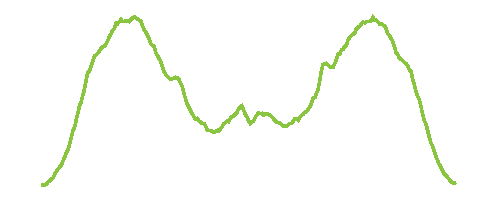
\includegraphics[width=0.1\textwidth]{ts_1.pdf}$))$};
	        
	        \node[inner sep=0pt] (ts1) at (4, 2.2)
	        {$c(g($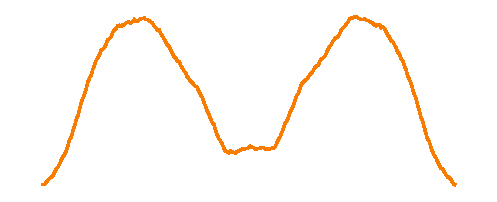
\includegraphics[width=0.1\textwidth]{ts_2.pdf}$))$};
	        
	        \node[inner sep=0pt] (ts1) at (8, 2.2)
	        {$c(g($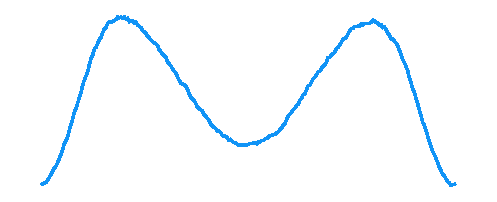
\includegraphics[width=0.1\textwidth]{ts_3.pdf}$))$};
			
    \end{tikzpicture}
\end{document}